% Options for packages loaded elsewhere
\PassOptionsToPackage{unicode}{hyperref}
\PassOptionsToPackage{hyphens}{url}

\documentclass[]{ctexart}
\usepackage{amssymb, amsmath}

\usepackage{geometry}
\usepackage{fancyhdr}
\pagestyle{fancy} 
\fancyfoot[R]{\thepage}
\fancyfoot[L]{\it 湖南大学课程}

\fancyhead[L]{\it《宏观经济学》}
\fancyhead[R]{\it 数字经济专业}

\fancyfoot[C]{}


\usepackage{hyperref}
\urlstyle{same} % disable monospaced font for URLs
\usepackage{longtable,  booktabs}

\usepackage{etoolbox}
\makeatletter
\patchcmd\longtable{\par}{\if@noskipsec\mbox{}\fi\par}{}{}
\makeatother
% Allow footnotes in longtable head/foot
\IfFileExists{footnotehyper.sty}{\usepackage{footnotehyper}}{\usepackage{footnote}}
\makesavenoteenv{longtable}
\usepackage{graphicx}
\makeatletter
\def\maxwidth{\ifdim\Gin@nat@width>\linewidth\linewidth\else\Gin@nat@width\fi}
\def\maxheight{\ifdim\Gin@nat@height>\textheight\textheight\else\Gin@nat@height\fi}
\makeatother
% Scale images if necessary,   so that they will not overflow the page
% margins by default,   and it is still possible to overwrite the defaults
% using explicit options in \includegraphics[width,   height,   ...]{}
\setkeys{Gin}{width=\maxwidth,  height=\maxheight,  keepaspectratio}
% Set default figure placement to htbp
\makeatletter
\def\fps@figure{htbp}
\makeatother
\setlength{\emergencystretch}{3em} % prevent overfull lines
\providecommand{\tightlist}{%
  \setlength{\itemsep}{0pt}\setlength{\parskip}{0pt}}
\setcounter{secnumdepth}{-\maxdimen} % remove section numbering


\begin{document}

\section*{IS-LM 的应用:  财政与货币政策分析}


\begin{itemize}
\item
  我们在凯恩斯交叉中分析了财政政策的影响. 主要结论是政府可以根据乘数效应,  用扩张性财政来刺激产出. 

  \begin{itemize}
  \item
    凯恩斯交叉中,  投资是外生给定的,  没有考虑利率对投资的影响,  也没有考虑货币市场. 
  \end{itemize}
\item
  现在,  我们用 IS-LM
  模型来分析财政政策和货币政策的效果. 由于乘数效应,  政府购买提高
  \(\Delta G\) 会使得 IS 曲线右移 \(\frac{1}{1 - MPC} \Delta G\).

  \begin{itemize}
  \item
    然而,  我们发现, 均衡利率也会提高,  这导致投资下降. 
    因此,   IS-LM 模型中政府购买对 GDP 的刺激作用比凯恩斯交叉中要小. 
  \end{itemize}
\end{itemize}

\subsubsection*{财政政策使 IS 曲线移动}

\textbf{一、当政府购买$G$提高 \(\Delta G\)时:} 

\begin{figure}
\centering
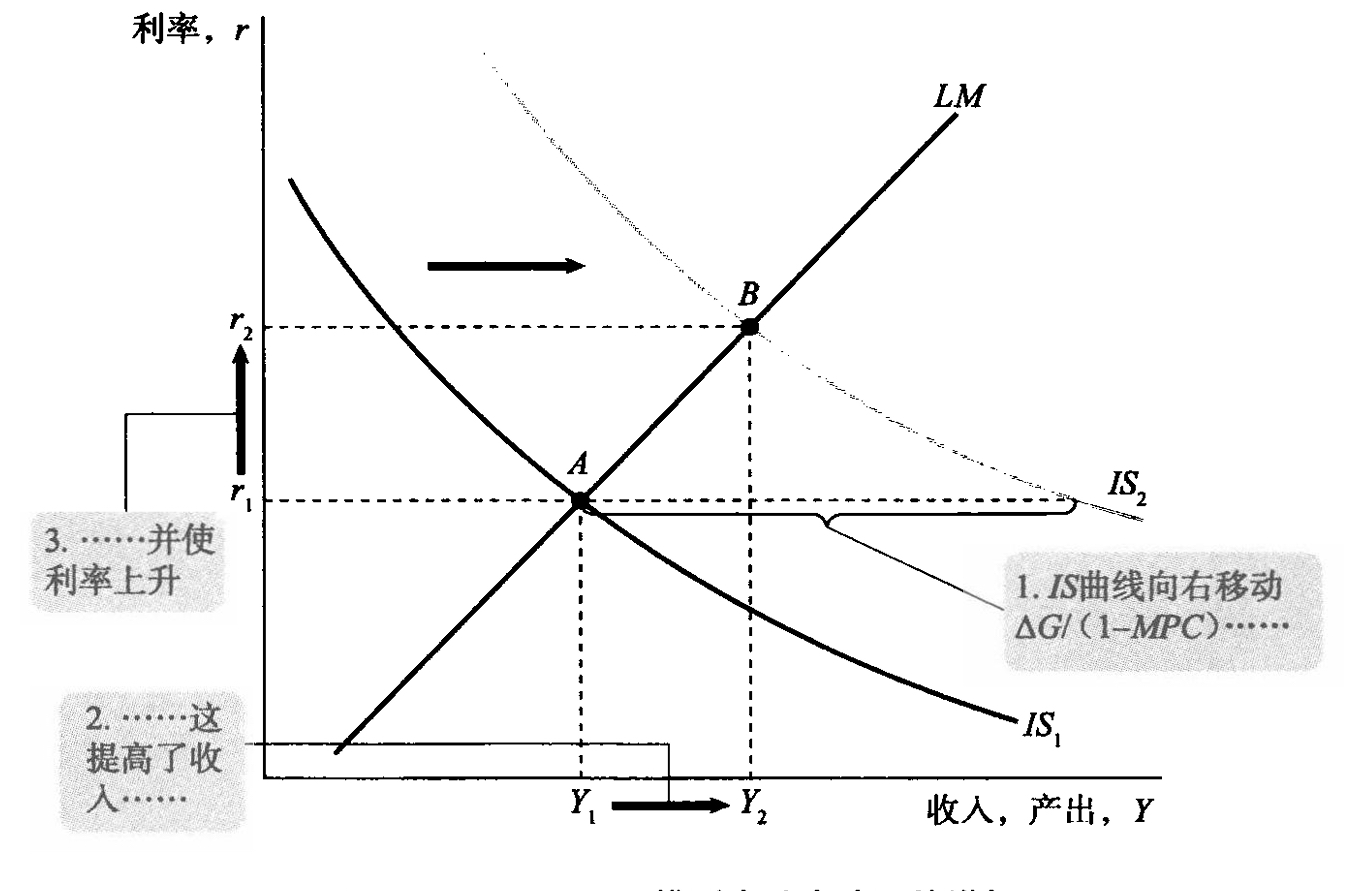
\includegraphics[width=0.6\textwidth]{fig2/is-1.jpeg}
\caption{宽松财政对 IS 的影响,  挤出效应}
\end{figure}


\begin{itemize}
\item
  凯恩斯交叉告诉我们,  在任何给定的利率 $r$ 下, 这都会使得产出增加
  \(\Delta Y= \frac{1}{1-MPC} \Delta G\). 因此, IS 曲线会右移
  \(\Delta Y\) 单位. 
\item
  同时,  由于 $Y$ 上升,  货币市场中居民对实际货币余额的需求也增加,  均衡利率上升. 但是,  这不会导致
  LM 曲线本身移动,  而是使均衡从点 A 沿着 LM 曲线变动到点 B.
\item
  由图 1 可知,  因为 LM 曲线向上倾斜,  均衡产出的变化 ( \(Y_2 - Y_1\) ) 小于
  \(\frac{1}{1-MPC} \Delta G\).

  \begin{itemize}
  \item
    政府购买会挤出家庭和企业投资,  这被称为\textbf{``挤出效应''}. 
  \end{itemize}
\end{itemize}

结论: 提高政府购买时, 均衡收入和均衡利率均上升. 
但由于存在挤出效应, 均衡收入的上升幅度比凯恩斯交叉模型的预测要少. 

\textbf{二、当政府将税收减少 \(\Delta T\)时:}

\begin{itemize}
\item
  类似上述分析,  这会使 IS 曲线右移 \(\frac{MPC}{1-MPC} \Delta T\),  LM 曲线则不移动. 
\item
  由于利率的提高抑制了投资, 均衡时收入的提高同样小于凯恩斯交叉模型的预测. 
\end{itemize}

\subsubsection*{货币政策使 LM 曲线移动}

\begin{itemize}
\item
  假设美国的央行 (美联储) 降低货币供给, 这会使实际货币余额市场的供给左移(图2a); 任意给定产出水平下, 货币市场的均衡利率均会上升, 因此 LM 曲线上移 (图2b). 
\end{itemize}

\begin{figure}
\centering
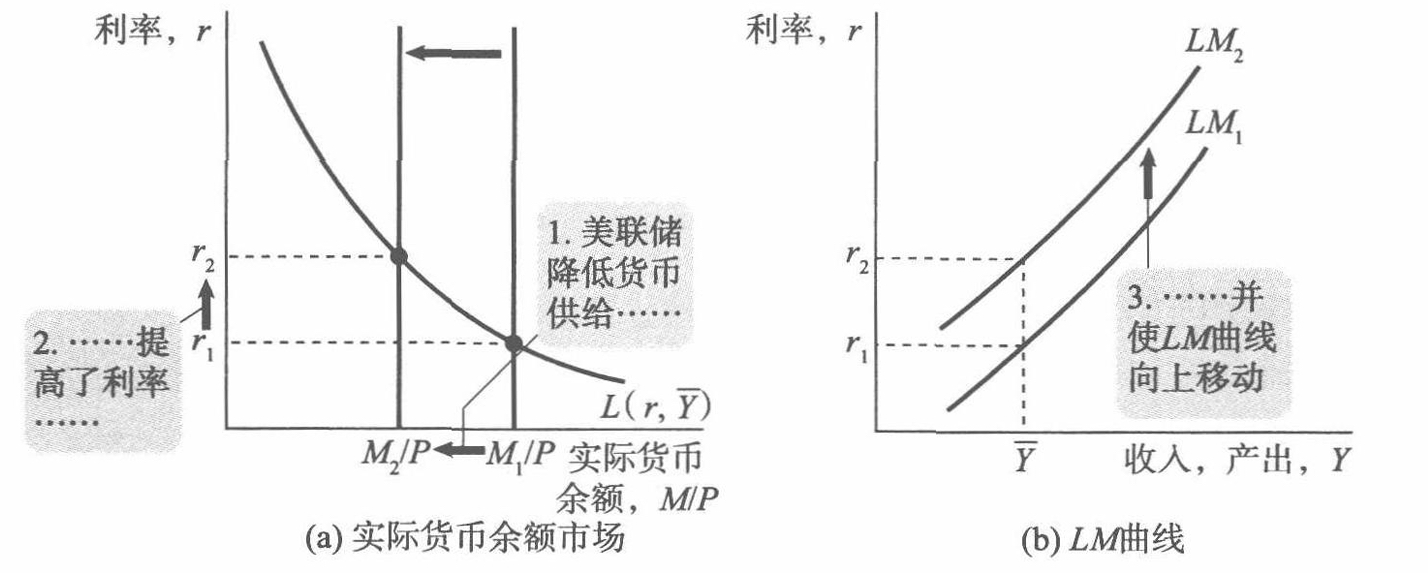
\includegraphics[width=0.8\textwidth]{fig2/lm-1.jpeg}
\caption{货币政策使 LM 曲线移动}
\end{figure}

\begin{itemize}
\item
  同理,  若提高货币供给, 则会降低任意产出水平下货币市场的均衡利率,  LM 曲线下移. 
\end{itemize}

\textbf{三、宽松货币政策的影响:} 

\begin{itemize}
\item
  LM 曲线下移,  均衡利率和产出均下降. (图3)
\end{itemize}

\begin{figure}
\centering
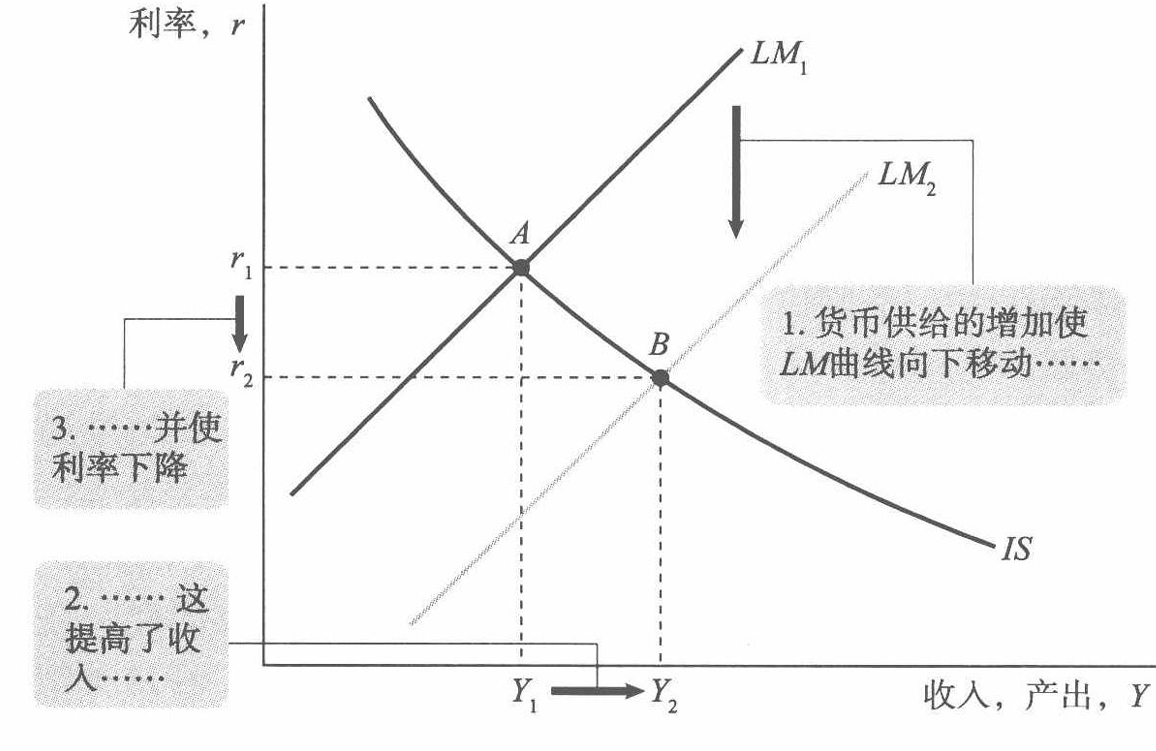
\includegraphics[width=0.6\textwidth]{fig2/lm-2.jpeg}
\caption{宽松货币政策的影响}
\end{figure}

图形分析的结果很直观,  但我们也要学会从流动性偏好理论入手,  用文字说明为什么增加货币供给会导致收入上升和利率下降. 

\begin{itemize}
\item
  当央行增加货币供给时, 居民会用这些额外的货币来购买其它金融资产(如债券), 这导致利率从
  \(r_1\) 降到 \(r_2\). 
  低利率进一步刺激了投资,  从而导致均衡产出上升. 
\end{itemize}


\paragraph{小结}
  \begin{longtable}[]{@{}lll@{}}
\toprule
政策 & 均衡收入 & 均衡利率\tabularnewline
\midrule
\endhead
宽松财政 (提高 G 或减少 T) & 上升 $\uparrow$ & 上升 $\uparrow$ \tabularnewline
宽松货币 (提高 M) & 上升 $\uparrow$ & 下降 $\downarrow$  \tabularnewline
\bottomrule
\caption{宽松财政政策和货币政策对经济的影响}
\end{longtable}

补充说明: 
\begin{enumerate}
\item 
  上述对货币政策的分析中,  我们都假设央行是通过控制名义货币供给 M 来影响 LM 曲线的.
\item 
  现实经济中, 央行有很多可选的货币政策工具.
  我们会在之后的第十五章(宏观经济政策)中讨论央行可用的货币政策工具, 如公开市场购买、调整存款准备金率等. 
\end{enumerate}

\newpage

\paragraph{货币与财政政策的共同作用}

\begin{itemize}
  \item 假设政府为了缓解赤字,  决定加税,  这会导致均衡收入和利率均下降. 此时,  政府还可以通过货币政策,  使得均衡利率或者收入不变. 

  \item 在很多国家,  财政政策由联邦政府决定,  而货币政策由央行决定. 并且, 央行独立于联邦政府, 具有很高的自主性.  央行可以在政府加税后,  用灵活的货币政策来决定是保利率(图4)还是保产出(图5). 
\end{itemize}

\begin{figure}
\centering
\begin{minipage}{.48\textwidth}
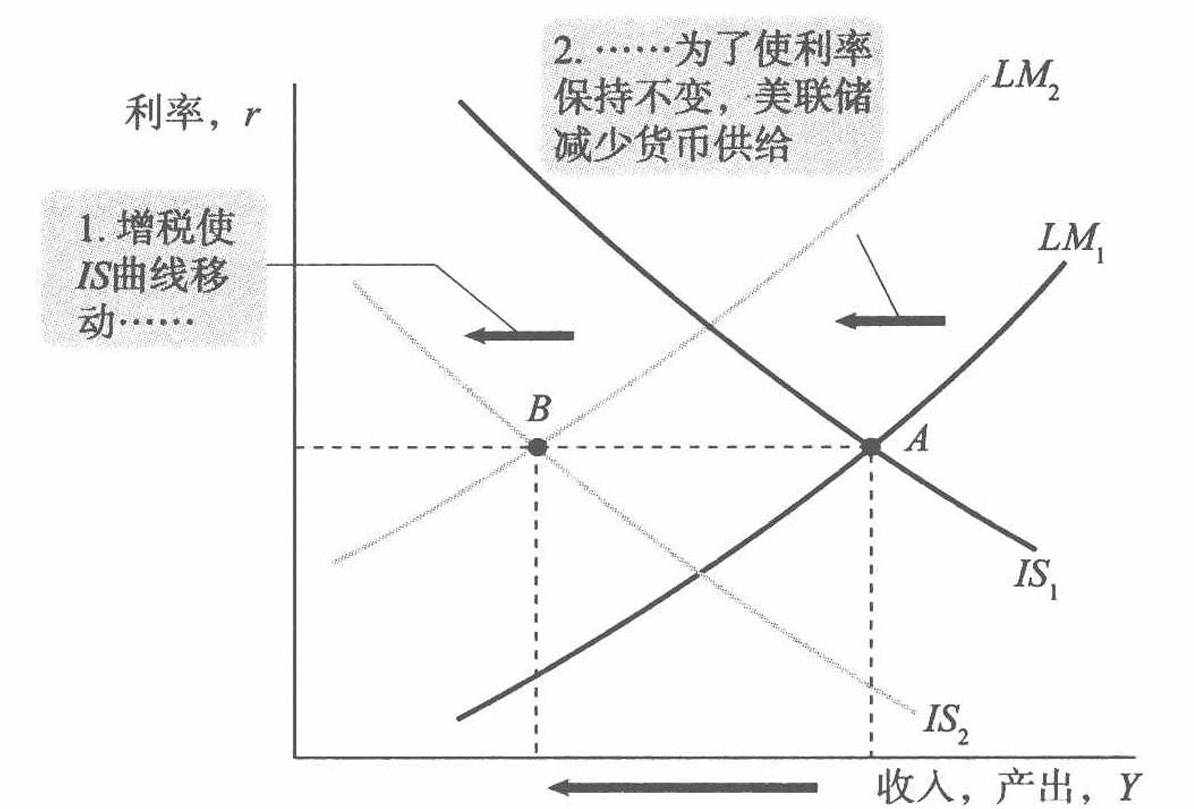
\includegraphics[width=0.9\textwidth]{fig2/is-lm1.jpg}
\caption{减少货币供给以维持利率}

\end{minipage}%
\begin{minipage}{.5\textwidth}

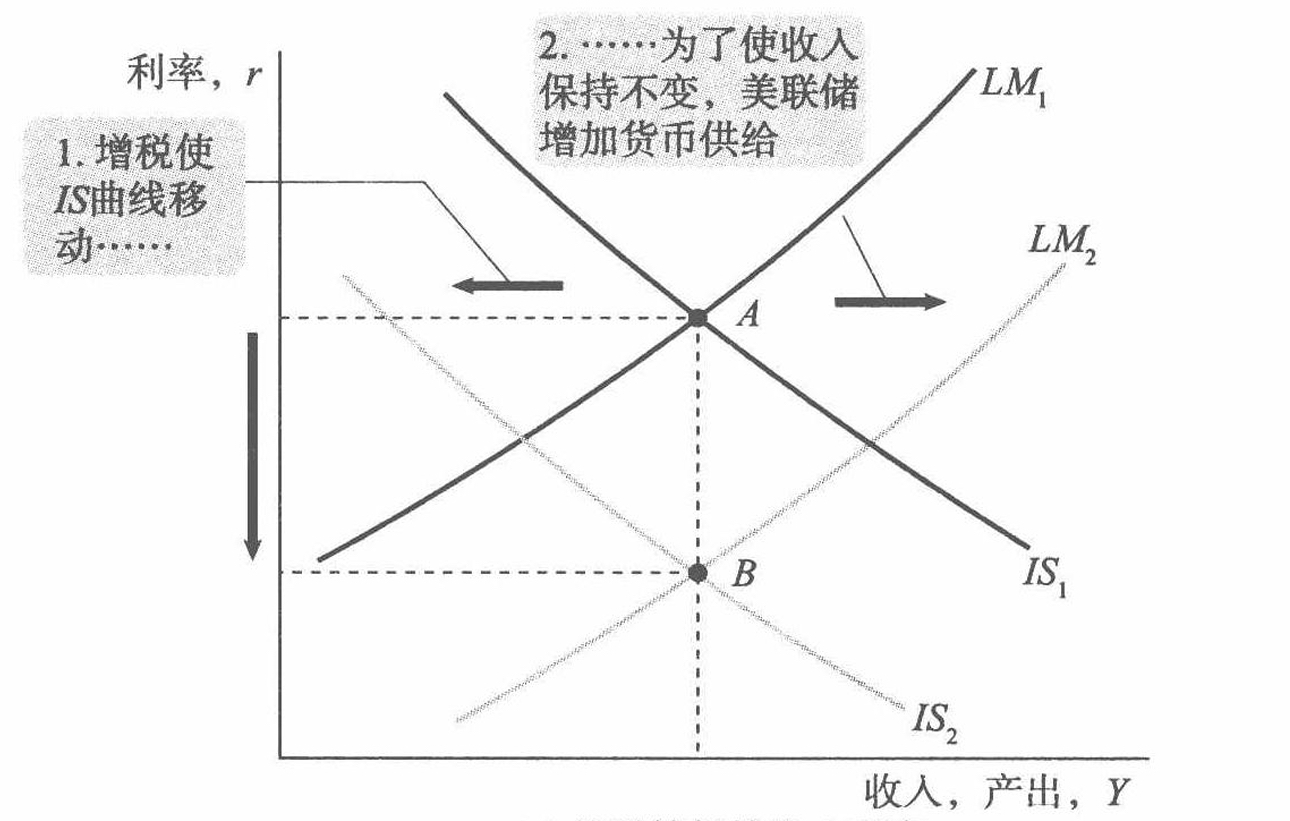
\includegraphics[width=0.9\textwidth]{fig2/is-lm2.jpeg}
\caption{增加货币供给以维持产出}


\end{minipage}
\end{figure}


\paragraph{其他冲击}

除了政府的财政政策和央行的货币政策外,  还有其他因素会使 IS 和 LM
曲线移动. 



\begin{enumerate}
\def\labelenumi{\arabic{enumi}.}
\item
  IS 的变动源于产品与服务市场需求的变化: 

  \begin{itemize}
  \item
    凯恩斯的动物精神 (animal spirits): 
    企业对未来突然变得悲观,  减少了投资,  IS 曲线左移. 
  \item
    家庭对消费品需求的变动: 
    一位受欢迎的领导人当选,  增强了人们对经济的信心,  消费上升,  IS
    曲线右移. 
  \end{itemize}
\item
  LM 的变动源于货币市场中需求的变动: 
  \begin{itemize}
  \item
    新兴金融创新产品 (如余额宝) 在带来投资回报的同时,   也提供了流动性. 这会减少人们的货币持有量. 根据流动性偏好理论,  货币需求下降时,  货币市场的均衡利率下降,  LM
    曲线下移,  这会使均衡收入上升. 
  \end{itemize}
\end{enumerate}

\paragraph{练习: }下列情况发生时,  
利率 $r$,   收入 $Y$,   消费 $C$ 和投资 $I$ 会如何变动?

1. 央行增加货币供给. 
2. 政府增加政府购买.
3. 政府增加税收.
4. 政府等量地增加 $G$ 和 $T$.

\end{document}
